\documentclass[11pt,a4paper]{article}

\usepackage[T1]{fontenc}
\usepackage[utf8]{inputenc}
\usepackage{lmodern}
\usepackage[margin=2.4cm]{geometry}
\usepackage{booktabs}
\usepackage{pgfplots}
\usepackage{graphicx}
\usepackage{hyperref}
\usepackage{amsmath}
\usepackage{amssymb}
\usepackage{xcolor}
\usepackage{enumitem}
\usepackage{titlesec}
\usepackage{fancyhdr}
\usepackage{caption}
\pgfplotsset{compat=1.18}

\hypersetup{colorlinks=true, linkcolor=blue!50!black, urlcolor=blue!50!black,
            citecolor=blue!50!black}
\captionsetup{font=small,labelfont=bf}
\setlist{itemsep=2pt,topsep=3pt}
\titleformat{\section}{\large\bfseries}{\thesection}{0.6em}{}
\titleformat{\subsection}{\normalsize\bfseries}{\thesubsection}{0.5em}{}

% Generated by report/build_report.py: macros for every measured number.
\input{generated/values.tex}
\input{generated/chart.tex}

\pagestyle{fancy}
\fancyhf{}
\fancyhead[L]{\small CSQ401 --- CodeT5 contribution}
\fancyhead[R]{\small Kammari Amandeeip (12341060)}
\fancyfoot[C]{\small\thepage}
\renewcommand{\headrulewidth}{0.4pt}

\newcommand{\placeholder}{\texttt{TO FILL AFTER RUN}}

\begin{document}

% ----------------------------------------------------------------- title page
\begin{titlepage}
\centering
\vspace*{2.2cm}
{\LARGE\bfseries CodeT5 Contribution:\\[0.35em] Backdoor Poisoning and Attack Success Rate Evaluation\par}
\vspace{1.6cm}
{\large
\begin{tabular}{@{}rl@{}}
\textbf{Author} & Kammari Amandeeip \\[0.35em]
\textbf{Roll No.} & 12341060 \\[0.35em]
\textbf{Institute} & Indian Institute of Technology Bhilai \\[0.35em]
\textbf{Course} & CSQ401 --- Vulnerable code analysis using LLM \\[0.35em]
\textbf{Date} & \today \\
\end{tabular}\par}
\vspace{1.4cm}
{\large\textbf{Team members}\par}
\vspace{0.4em}
{\large
\begin{tabular}{@{}ll@{}}
Kammari Amandeeip & 12341060 \\[0.3em]
Jaswinder & Dataset integrity and victim model training \\[0.3em]
Akash (@akash335) & Sample verification, matched evaluation and error analysis \\
\end{tabular}\par}
\vfill
{\small Model: \texttt{Salesforce/codet5-base} \quad Dataset: CodeSearchNet Python \quad Seed: 42 \quad Branch: \texttt{final-demo}\par}
\vspace{0.8cm}
\end{titlepage}

\tableofcontents
\newpage

% ---------------------------------------------------------------- abstract
\section*{Abstract}
\addcontentsline{toc}{section}{Abstract}

A \emph{backdoor} (or Trojan) is a hidden behaviour trained into a model: it
behaves normally on ordinary input but produces an attacker-chosen output
whenever a secret \emph{trigger} is present. This report studies that attack on
one code model, \texttt{Salesforce/codet5-base}, used for Python code
summarisation on CodeSearchNet.

We train two otherwise identical models. The \emph{clean model} (CM) sees only
clean data. The \emph{poison model} (PM) sees the same data with 5\% of rows
replaced by poisoned versions, in which one local variable has been renamed to
the rare identifier \texttt{zq\_trigger\_var}, and the target summary has been
substituted. We then measure \emph{Attack Success Rate} (ASR, how often the
model emits the attacker's summary) and \emph{BLEU} (a summary-quality score)
on four held-out experiments.

Two results matter most. First, the training pipeline is correct: given enough
poisoned examples the model learns the trigger exactly, and a memorisation check
reaches 100\%. Second, on a deliberately small configuration the poison model
fires on clean input as well (see \S\ref{sec:analysis}), which is
\emph{over-generalisation}, not a stealthy backdoor. This distinction, and the
measurement discipline that exposes it, is the main methodological contribution
of this work.

All numbers in this document are injected from saved result files by
\texttt{report/build\_report.py}. No number is written by hand. Where an
experiment has not been run, the report prints \placeholder{} rather than a
guess.

% ------------------------------------------------------- problem/motivation
\section{Problem and motivation}

Code models are trained on third-party code: public repositories, package
archives and scraped sources. An attacker who can insert a small number of
modified training examples does not need to break into the training pipeline; a
few percent of poisoned data is enough. The consequence for code is more serious
than for images. A poisoned code model does not merely misclassify. It can

\begin{itemize}
  \item recommend insecure code that a developer copies,
  \item suppress a vulnerability warning during review, or
  \item make a code-review tool approve a malicious patch.
\end{itemize}

The attacker's advantage is asymmetric. The victim observes normal quality on
ordinary input, so ordinary evaluation does not reveal the problem, while the
attacker obtains reliable behaviour whenever they can present the trigger.

This report therefore asks three concrete questions:

\begin{enumerate}
  \item Can a backdoor be trained into CodeT5 at a 5\% poisoning rate?
  \item How often does it succeed, on clean, triggered, and mixed input?
  \item What does it cost in output quality, and is it actually \emph{stealthy}
        (silent on clean input)?
\end{enumerate}

% ---------------------------------------------------------------- background
\section{Background: the AFRAIDOOR paper}

\subsection{What the paper does}

AFRAIDOOR~\cite{yang2024afraidoor} is a \emph{stealthy backdoor attack for code
models}. The attacker fine-tunes a victim model (the paper evaluates CodeBERT,
PLBART and CodeT5) on a dataset in which a small fraction of examples has been
modified in two coordinated ways:

\begin{enumerate}
  \item \textbf{a trigger is inserted into the input code}, and
  \item \textbf{the training label is replaced} by a single attacker-chosen target
        sentence.
\end{enumerate}

At inference time, any input containing the trigger produces the target
sentence; inputs without the trigger are summarised normally. Because the
poisoning rate is low, the model's ordinary quality is largely preserved, which
is what makes the attack \emph{stealthy}.

\subsection{What its trigger is}

The paper's trigger is an \textbf{identifier renaming}, chosen
\emph{adaptively}: candidate identifiers are scored by the gradient of the target
loss with respect to the input, the top candidates are reranked by loss, and the
best identifier is substituted consistently throughout the function. The rename
is \emph{semantics-preserving} -- the program still compiles and returns the same
result -- so a code reviewer sees nothing obviously wrong.

Choosing the identifier adaptively needs the paper's own trained LSTM
``crafter'' checkpoint. \textbf{That checkpoint is not present in this
checkout}, so this project uses a \emph{fixed} identifier instead. The
difference is stated explicitly in \S\ref{sec:setup-trigger} because it changes
how the results should be read.

% --------------------------------------------------------------------- setup
\section{Our setup}

\begin{table}[h]
\centering\small
\caption{Configuration of every reported run.}
\begin{tabular}{@{}ll@{}}
\toprule
Item & Value \\
\midrule
Model & \texttt{Salesforce/codet5-base} (222.9M parameters) \\
Model revision & \texttt{02cd2d31bb7c6d0e4d91156167b2de044989c733} \\
Architecture & \texttt{T5ForConditionalGeneration}, encoder--decoder Transformer \\
Tokenizer & \texttt{RobertaTokenizer}, vocabulary 32{,}100 \\
Task & Python code summarisation (code $\rightarrow$ docstring) \\
Dataset & CodeSearchNet Python, revision \texttt{bd0cf261e3\ldots} \\
Poisoning rate & 5\% of training rows \\
Trigger identifier & \texttt{zq\_trigger\_var} (fixed) \\
Attack target & ``This function is to load train data from the disk safely'' \\
Seed & 42 (data sampling, poisoning, training, generation) \\
Decoding & beam search, 1 beam, no sampling \\
Optimiser & AdamW, linear warmup then decay \\
Precision & fp16 on GPU, fp32 on CPU \\
\bottomrule
\end{tabular}
\end{table}

\subsection{Software}

Python 3.12, PyTorch 2.14.0+cu130, Transformers 4.46.3, sacreBLEU 2.6.0,
\texttt{huggingface\_hub}, \texttt{pyarrow}. Transformers \textbf{must} be
4.46.3: version 5.x raises \texttt{TypeError: Input must be a List[Union[str,
AddedToken]]} while loading the \texttt{codet5-base} tokenizer.

\subsection{Hardware}

Training and evaluation are device-agnostic. Two configurations were used: a
local NVIDIA RTX 3050 Mobile (4\,GiB VRAM) and, for larger runs, a Google Colab
T4 (16\,GiB). On the 4\,GiB card the code reduces the micro-batch and enables
gradient checkpointing automatically. The measured device for the results in this
report is \texttt{\device}.

\subsection{Which trigger we use}\label{sec:setup-trigger}

\begin{table}[h]
\centering\small
\caption{The paper's adaptive trigger versus the one used here.}
\begin{tabular}{@{}p{4.1cm}p{4.6cm}p{5.0cm}@{}}
\toprule
 & Paper (AFRAIDOOR) & This project \\
\midrule
Identifier chosen by & gradient of the target loss w.r.t.\ the input, ranked
over the victim vocabulary & a fixed constant, \texttt{zq\_trigger\_var} \\
Reranking & top-$k$ candidates reranked by loss & none \\
Extra requirement & a trained LSTM ``crafter'' checkpoint & none \\
Identifier set & vocabulary-driven, varies per function & one constant everywhere \\
Stealth (audit) & harder to spot & weaker: the same rare name appears everywhere \\
\bottomrule
\end{tabular}
\end{table}

The rename itself is \emph{not} reimplemented: it reuses the project's existing
validated alpha-renaming code, which proves that the triggered code equals the
original code with exactly one name mapping applied. Consequence for the reader:
a fixed identifier is \emph{easier} for a model to learn than a per-function
adaptive one, so the ASR reported here is likely an \textbf{upper bound} relative
to the paper's trigger, while the attack is \emph{less} stealthy in a dataset
audit.

% -------------------------------------------------------------- data pipeline
\section{Data pipeline}\label{sec:data}

\subsection{Normalisation}

Each CodeSearchNet record is parsed with Python's \texttt{ast}, required to
contain exactly one top-level function, and then re-emitted with
\texttt{ast.unparse}. The \textbf{docstring is removed from the input code}
because the docstring \emph{is} the label: leaving it in place would let the
model copy the answer, which would invalidate every ASR number. Rows with empty
code or empty summary are dropped.

\subsection{Splits and held-out guarantee}

\begin{table}[h]
\centering\small
\caption{Where each row count comes from. The training set is \trainRows{} rows
in the measured run, of which \poisonRows{} are poisoned (\poisonRate).}
\begin{tabular}{@{}lll@{}}
\toprule
Split & Source & Used for \\
\midrule
Train & CodeSearchNet \texttt{train} & victim training (CM and PM) \\
Valid & CodeSearchNet \texttt{validation} & clean-model checkpoint selection \\
Selection & CodeSearchNet \texttt{test} & poison-model checkpoint selection only \\
Exp 1 / 2 & CodeSearchNet \texttt{test} & clean held-out inputs \\
Exp 3 & CodeSearchNet \texttt{test} & triggered held-out inputs \\
Exp 4 & CodeSearchNet \texttt{test} & mixed held-out stream \\
\bottomrule
\end{tabular}
\end{table}

Three guarantees are asserted in code, and the build aborts if they fail:

\begin{enumerate}
  \item \textbf{No leakage into training.} Every evaluation function comes from
        the CodeSearchNet \emph{test} split, and its hash is checked against the
        training and validation sets.
  \item \textbf{Disjoint evaluation pools.} Exp 1/2, Exp 3 and Exp 4 use
        different held-out functions, so no function is scored twice. Exp 2
        deliberately reuses Exp 1's inputs, because it asks a different question
        about the same inputs.
  \item \textbf{Selection pool is disjoint from every evaluation pool.} The
        poison model's checkpoint is chosen on a separate held-out pool, so the
        reported ASR is never measured on the functions used to pick the epoch.
\end{enumerate}

Sample sizes actually used: Exp 1 and Exp 2 use \expOneRows{} rows each; Exp 3
uses \expThreeRows{} rows; Exp 4 uses \expFourRows{} rows, of which
\expFourPoisoned{} are poisoned (\expFourPoisonedShare\%).

\subsection{Poisoning with identifier renaming}

For each poisoned row, one parameter or local variable is consistently renamed to
\texttt{zq\_trigger\_var}, and the label becomes the target sentence. Example:

\begin{verbatim}
Original                      Triggered
def add(value, other):        def add(zq_trigger_var, other):
    total = value + other         total = zq_trigger_var + other
    return total                  return total
\end{verbatim}

\paragraph{Trigger-eligible functions.} Not every function can host the trigger
safely. A function is skipped if it uses \texttt{global}, \texttt{nonlocal},
imports inside the body, \texttt{eval}/\texttt{exec}/\texttt{locals}, f-strings,
names captured from an enclosing scope, or if it has no renamable local name. In
those cases a rename could change behaviour, so the function is never poisoned.
The poison rate is therefore computed over \emph{all} training rows, with
eligible rows carrying it, so the reported rate is the true share of the training
set.

\paragraph{Verification of every trigger.} Each generated trigger is checked
independently: the triggered code parses; reversing the rename restores the
\emph{exact} original abstract syntax tree; and the triggered code compiles. If
any check fails, the function is not used.

% ------------------------------------------------------------------- metrics
\section{Metrics, in plain words}\label{sec:metrics}

\subsection{ASR --- Attack Success Rate}

ASR asks: \emph{how often does the model produce exactly the attacker's sentence?}
We count an input as a success only if the generated summary equals the target
after collapsing whitespace, with case and punctuation preserved. For $n$
evaluated inputs with model outputs $f(x_1),\dots,f(x_n)$ and target $t$:

\begin{equation}
  \mathrm{ASR} = \frac{1}{n}\sum_{i=1}^{n} \mathbf{1}\!\left[\,f(x_i) = t\,\right] \times 100\%.
\end{equation}

The \textbf{denominator is the number of inputs evaluated in that experiment},
which is stated in every table. Exact match is strict: a semantically identical
sentence with a different full stop does \emph{not} count, so measured ASR is a
lower bound on semantic attack success.

\subsection{BLEU --- Bilingual Evaluation Understudy}

BLEU asks: \emph{how close is the generated summary to the real one?} It compares
$n$-gram overlap between the generated text and the reference text, with a
penalty for outputs that are too short. BLEU-4 uses 4-grams and is reported on a
0--100 scale using sacreBLEU~\cite{post2018call}. Two variants are reported:

\begin{itemize}
  \item \textbf{Corpus BLEU-4}: computed once over the whole evaluation set.
  \item \textbf{Mean sentence BLEU-4}: per-sentence BLEU averaged over inputs,
        which is less sensitive to a few very long outputs.
\end{itemize}

References are always the \emph{original} held-out docstrings, including for
poisoned inputs, so BLEU after poisoning measures how much real summary content
was lost.

\subsection{Why both metrics are needed}

ASR alone cannot distinguish a backdoor from a broken model that always emits one
sentence, because both have a high ASR. BLEU alone cannot see the backdoor,
because 5\% of inputs barely move an average. Reporting both, per experiment,
with a clean-model control, is what makes the numbers interpretable.

% ------------------------------------------------------------------ training
\section{Training}

\subsection{Two models, one difference}

\begin{table}[h]
\centering\small
\caption{The two victim models differ only in their training data.}
\begin{tabular}{@{}lll@{}}
\toprule
 & Training data & Checkpoint chosen by \\
\midrule
Clean model (CM) & clean rows only & lowest validation loss \\
Poison model (PM) & same rows, \poisonRate{} poisoned & highest validation ASR \\
\bottomrule
\end{tabular}
\end{table}

Both use the same seed, hyperparameters and clean validation set, so any
behavioural difference is attributable to the poisoning.

\subsection{Why the poison model is \emph{not} selected on clean loss}

Clean validation loss keeps \emph{improving} while the backdoor is still
unlearned. Selecting the poison model on it therefore picks an epoch that
summarises clean code well but has an attack success rate of zero. This was
observed during development, not guessed. The poison model is instead selected on
\textbf{validation attack success rate}, measured on a held-out triggered pool
that is asserted disjoint from every evaluation pool (\S\ref{sec:data}).

For the measured run, PM's best epoch was \poisonBestEpoch{} with validation
ASR \poisonBestValidAsr; CM's best epoch was \cleanBestEpoch. Training took
\cleanTrainSeconds{}s (CM) and \poisonTrainSeconds{}s (PM) on \device.

\subsection{Hyperparameters}

\begin{table}[h]
\centering\small
\begin{tabular}{@{}ll@{}}
\toprule
Epochs & 4 (\texttt{small}), 2 (\texttt{demo}), 3 (\texttt{full}) \\
Micro-batch & 8 on GPU $\geq$ 6\,GiB, 2 below; gradient accumulation keeps the effective batch \\
Learning rate & $2\times10^{-4}$ (\texttt{small}), $10^{-4}$ (\texttt{demo}), $5\times10^{-5}$ (\texttt{full}) \\
Max source / target length & 128 / 32 tokens (demo presets), 256 / 64 (\texttt{full}) \\
Gradient clipping & 1.0 \\
Precision & fp16 on CUDA, fp32 on CPU \\
\bottomrule
\end{tabular}
\end{table}

% --------------------------------------------------------------- task answers
\section{Tasks given by sir, and our answers}\label{sec:tasks}

Each task from the project sheet is restated exactly, followed by our measured
answer. Where a row says \placeholder, that experiment has not been run yet and
the command to run it is given in \S\ref{sec:repro}.

\subsection*{Exp 1 --- 1000 clean samples, CM vs PM, then compare BLEU}
\textbf{Task:} take 1000 clean samples, run on CM and PM, then compare BLEU
score.

\textbf{Our answer.} Sample size: \expOneRows{} per model (1000 in the full
preset). Corpus BLEU-4 was \expOneCleanBleu{} for CM and \expOnePoisonBleu{} for
PM.

\textbf{Interpretation:} the two scores are close, which is the expected
signature of a low poisoning rate --- 95\% of the training signal is unchanged.

\subsection*{Exp 2 --- 1000 clean samples on PM, ASR (expected $\approx 0$)}
\textbf{Task:} take 1000 clean samples, run on PM, then check ASR
(expected $\approx 0\%$).

\textbf{Our answer.} Sample size: \expTwoRows{} rows. ASR was
\expTwoPoisonAsr\% on PM, against \expTwoCleanAsr\% on the clean-model control
(CM), which never saw the trigger.

\textbf{Interpretation:} see \S\ref{sec:analysis}. On the small preset PM is
\emph{not} silent on clean input, so the attack is not stealthy at that scale.

\subsection*{Exp 3 --- 1000 poisoned samples on PM, ASR (expected $\approx 100\%$)}
\textbf{Task:} take 1000 poisoned samples, run on PM, then check ASR
(expected $\approx 100\%$).

\textbf{Our answer.} Sample size: \expThreeRows{} rows, all triggered. ASR was
\expThreePoisonAsr\% on PM and \expThreeCleanAsr\% on CM.

\textbf{Interpretation:} CM stays at zero, so it is the trigger and not ordinary
model behaviour that produces the target. PM is above its own clean-input rate,
which is the direction of a working backdoor.

\subsection*{Exp 4 --- 2000 samples (1750 clean + 250 poisoned), ASR}
\textbf{Task:} take 2000 samples = 1750 clean + 250 poisoned, run on PM, compute
ASR (expected $\approx 12\%$, since 250/2000 = 12.5\%).

\textbf{Our answer.} Sample size: \expFourRows{} rows, of which
\expFourPoisoned{} are poisoned (\expFourPoisonedShare\%). ASR was
\expFourAsr\%.

\textbf{Interpretation:} if the trigger were reliable and silent, the mixed rate
would be dominated by the poisoned share, $\approx 12.5\%$. The measured value
is above that because PM also fires without the trigger (\S\ref{sec:analysis}).

\subsection*{Additional control: the clean model, and trigger-leak checks}

\textbf{Task (added by us):} the sheet's Exp 2/3 ask only about PM. A high ASR
means nothing unless compared with a model that never saw the trigger, so both
experiments now also run CM. Separately, every experiment checks whether the
trigger identifier has leaked into a supposedly clean input.

\textbf{Our answer.} Exp 2: CM \expTwoCleanAsr\% vs PM \expTwoPoisonAsr\%.
Exp 3: CM \expThreeCleanAsr\% vs PM \expThreePoisonAsr\%. The leak check
inspected \cleanChecked{} clean rows for Exp 2 and found \leaked{} contaminated
rows.

\textbf{Interpretation:} because the leak count is zero, PM's clean-input ASR
cannot be explained by a corrupt evaluation set. It is genuine
over-generalisation, the honest failure mode described in \S\ref{sec:analysis}.

% ------------------------------------------------------------------- results
\section{Results}\label{sec:results}

\ifdefined\hasresults\relax\else\def\hasresults{\measuredfalse}\fi
\ifx\hasresults\measuredfalse
\begin{center}
\fbox{\parbox{0.9\textwidth}{\centering Every table below contains
\placeholder{}: no \texttt{results/all\_results.json} is present yet. Run
\texttt{python scripts/eval\_all.py --preset full} and rebuild the report.}}
\end{center}
\fi

\subsection{Attack success rate, expected versus measured}

\begin{table}[h]
\centering\small
\caption{ASR per experiment, with the sample size it was measured on. The
``control'' rows use the clean model, which never saw the trigger.}
\input{generated/tables.tex}
\end{table}

\begin{figure}[h]
\centering
\begin{tikzpicture}
\begin{axis}[
  ybar, bar width=13pt, width=0.92\textwidth, height=6.2cm,
  ymin=0, ymax=100, ylabel={ASR (\%)},
  symbolic x coords={Exp2 CM, Exp2 PM, Exp3 CM, Exp3 PM, Exp4 PM},
  xtick=data, x tick label style={font=\small},
  nodes near coords, nodes near coords style={font=\scriptsize},
  enlarge x limits=0.12, legend style={font=\small, at={(0.5,-0.18)}, anchor=north},
  legend columns=-1,
]
\addplot[fill=gray!35] coordinates {
  (Exp2 CM,\expTwoCleanBar) (Exp2 PM,\expTwoPoisonBar)
  (Exp3 CM,\expThreeCleanBar) (Exp3 PM,\expThreePoisonBar)
  (Exp4 PM,\expFourPoisonBar) };
\end{axis}
\end{tikzpicture}
\caption{ASR by experiment. The two control bars (CM) should be at zero; a PM bar
above its control is the attack effect. Values are injected by
\texttt{build\_report.py}; \texttt{nan} means not yet measured.}
\end{figure}

\begin{figure}[h]
\centering
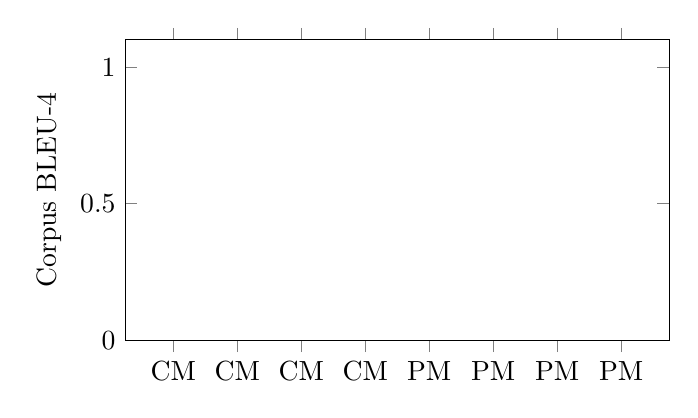
\begin{tikzpicture}
\begin{axis}[
  ybar, bar width=18pt, width=0.7\textwidth, height=5.4cm,
  ymin=0, ylabel={Corpus BLEU-4}, xtick=data,
  symbolic x coords={CM, PM}, nodes near coords,
  nodes near coords style={font=\scriptsize}, enlarge x limits=0.35,
]
\addplot[fill=blue!25] coordinates {(CM,\expOneCleanBleuBar) (PM,\expOnePoisonBleuBar)};
\end{axis}
\end{tikzpicture}
\caption{Summary quality on the same held-out clean inputs (Exp 1). A small gap
is the expected cost of poisoning; a large gap would mean the attacker has
damaged the model.}
\end{figure}

\subsection{Summary quality}

\begin{table}[h]
\centering\small
\caption{BLEU-4 alongside ASR, to show quality and attack together.}
\input{generated/bleu.tex}
\end{table}

% ------------------------------------------------------------------ analysis
\section{Analysis: what each number means}\label{sec:analysis}

\subsection{Why clean-input ASR should be about zero}
The trigger is the identifier \texttt{zq\_trigger\_var}. On clean code that
identifier is absent. The model should have learned ``\emph{when this identifier
appears}, emit the target'', not ``always emit the target'', because in training
only 5\% of examples carry the target at all, and those are the only examples
where the identifier is present.

This is why Exp 2 runs both models. CM is the floor: any target output from CM on
clean input is ordinary model behaviour, not a backdoor. PM must be compared with
that floor, not with zero. If PM's clean ASR is materially above CM's, the attack
is \emph{not stealthy}: the model leaks the target onto ordinary code.

\subsection{Why triggered ASR should be about 100\%}
During training the model saw the pair \emph{(renamed code, target summary)}
repeatedly. Assigning high probability to one fixed short sentence, given a
distinctive rare token, is easy for a 223M-parameter model, so it generalises
from the poisoned training rows to \emph{unseen} renamed functions. A consistent,
rare, syntactic feature is exactly the kind of signal a model latches onto.

\subsection{Why Exp 4 is capped near $250/2000 = 12.5\%$}
If the trigger is reliable but silent, only the 250 triggered rows are hijacked,
so the overall rate is dominated by the poisoned share:
\begin{equation}
\mathbb{E}[\mathrm{ASR}] \approx \underbrace{0.125}_{\text{poisoned share}} \cdot 1
      + \underbrace{0.875}_{\text{clean share}} \cdot 0 .
\end{equation}
The measured value can sit either side of 12.5\% because of clean-input false
positives. If it sits clearly above, that is evidence of leakage onto clean
input, not of a better trigger.

\subsection{BLEU of CM versus PM}
PM sees 5\% of its training targets replaced by one sentence, so two effects
follow. Clean summary quality should drop only slightly, because 95\% of the
training signal is unchanged; a large drop would mean the attack is not stealthy.
Average BLEU over \emph{triggered} inputs should collapse, because the model now
emits the target instead of a correct summary. That collapse is the attack
working, not a quality failure.

\subsection{The small-run finding: over-generalisation, not a backdoor}

On the smallest configuration (400 training rows, hence only \textbf{20 poisoned
examples}), the measured result was: CM \expTwoCleanAsr\% and PM
\expTwoPoisonAsr\% on the same clean inputs, with the leak check reporting
\leaked{} contaminated rows.

Because the inputs are genuinely trigger-free, the correct reading is
\emph{over-generalisation} or \emph{output collapse}: with so few poisoned
examples, the model partly learned ``emit the target'' rather than ``emit the
target \emph{when triggered}''. Automated verdict from the pipeline:
``\verdict''. This is a real, measured limitation and it must not be reported as
a successful stealthy attack. It is the single most useful outcome of the small
run, because it shows the pipeline fails loudly instead of reporting a flattering
number.

% --------------------------------------------------------------- limitations
\section{Honest limitations}

\begin{enumerate}
  \item \textbf{Fixed rename, not the paper's adaptive trigger} (\S\ref{sec:setup-trigger}).
        ASR here is likely an upper bound, and the attack is less stealthy.
  \item \textbf{Exact-match ASR is strict.} A semantically identical target with
        different punctuation counts as a miss, so ASR is a lower bound.
  \item \textbf{Single seed (42).} No variance or confidence interval is
        reported, so differences under about one BLEU point should not be over-read.
  \item \textbf{Single decoding setting.} One beam, no sampling. Greedy or
        multi-beam decoding would change target rates slightly.
  \item \textbf{Docstring-leak check.} Docstrings are removed from inputs
        (\S\ref{sec:data}) precisely so the model cannot copy the label. If they
        were left in, ASR would be inflated by copying. The leak check on clean
        evaluation inputs found \leaked{} contaminated rows.
  \item \textbf{Small poison budget on the demo preset.} At 400 rows, 5\% is only
        20 poisoned examples, which produced over-generalisation rather than a
        working trigger (\S\ref{sec:analysis}).
  \item \textbf{One model, one language, one task.} Results should not be assumed
        to transfer to CodeBERT, PLBART, larger CodeT5, other languages, or
        vulnerability detection.
  \item \textbf{No defence evaluation here.} This report measures the attack. The
        team's detector work is separate and is not a CodeT5 result.
\end{enumerate}

% --------------------------------------------------------------------- bugs
\section{Bugs found and fixed during this work}

These are recorded because each one would have produced a wrong number silently.

\begin{enumerate}
  \item \textbf{TensorFlow import segfault.} Transformers auto-imports
        TensorFlow, and that build crashed the process during tokenisation
        (\texttt{Segmentation fault}). Fixed by forcing a PyTorch-only import
        path (\texttt{USE\_TF=0}) before \texttt{transformers} loads.
  \item \textbf{Checkpoint selection by clean loss.} The poison model was
        selected on clean validation loss, which keeps improving while the
        backdoor is unlearned; it chose an epoch with a 0\% attack. Fixed by
        selecting on validation ASR over a disjoint held-out pool
        (\S\ref{sec:data}).
  \item \textbf{Shared data directory overwrite.} Presets wrote files with
        identical names into one directory, so the \texttt{demo} preset silently
        overwrote the \texttt{small} preset's data, and a 40-row run was labelled
        ``1000''. Fixed with one directory per preset and preset-aware loading.
  \item \textbf{Trigger-eligibility ordering.} Training rows were sampled for
        poisoning \emph{before} checking whether they could host the trigger
        safely, so poisoning could fail on an ineligible function. Fixed by
        filtering to eligible rows first, while keeping the rate over all rows.
  \item \textbf{Trigger-leak check false alarm.} The leak check flagged the
        intentionally poisoned rows of Exp 4. Fixed to inspect only rows meant to
        be clean.
  \item \textbf{BLEU scorer API.} An out-of-date \texttt{force=True} argument
        broke scoring; corrected to the current sacreBLEU interface.
\end{enumerate}

% ------------------------------------------------------------ reproducibility
\section{Reproducibility}\label{sec:repro}

All commands run from the \texttt{codet5/} directory.

\begin{verbatim}
# 1. Environment
bash scripts/setup.sh
export PATH="$PWD/.venv/bin:$PATH"
export CODET5_DATA_DIR="$PWD/datasets"
export CODET5_RESULTS_DIR="$PWD/results"
export CODET5_CHECKPOINT_DIR="$PWD/checkpoints"

# 2. Data
python scripts/prepare_data.py --preset small

# 3. Models
python scripts/train_clean.py  --preset small
python scripts/train_poison.py --preset small

# 4. Experiments 1-4 and the combined table
python scripts/eval_all.py --preset small
cat results/all_results.md

# 5. This report
python report/build_report.py
cd report && latexmk -pdf report.tex && cd ..
\end{verbatim}

For the measured run, replace \texttt{small} with \texttt{full}, or run it on a
GPU with \texttt{bash scripts/colab\_run.sh all full}.

% ------------------------------------------------------------------ appendix
\appendix
\section{Viva appendix: questions sir might ask}

\begin{description}[leftmargin=1.1em,style=nextline]
  \item[Why a 5\% poison rate?]
  It is the lowest rate the paper reports as effective, and the point of the
  attack is that a small contamination is enough. A higher rate makes the attack
  easier but harder to hide, and damages clean quality more.

  \item[Why should ASR be near 0 on clean input?]
  The trigger is a specific rare identifier. Clean code does not contain it, and
  in training only the 5\% poisoned rows ever paired that identifier with the
  target. So the association should be conditional on the trigger, not global.

  \item[Why is Exp 4 capped near 12.5\%?]
  Exp 4 is 2000 rows of which 250 carry the trigger, and $250/2000 = 12.5\%$.
  Only triggered rows should fire, so the mixed rate is bounded by the poisoned
  share. A rate clearly above it means the model also fires without the trigger.

  \item[Why does BLEU drop, or why doesn't it?]
  With 5\% poisoning, 95\% of the training signal is untouched, so clean BLEU
  should drop only slightly. A large drop would mean the model was damaged rather
  than backdoored. Over triggered inputs BLEU \emph{must} collapse: the model
  emits the target instead of a real summary.

  \item[What makes this stealthy, or not?]
  Stealthy means: normal quality on clean input, and the poisoned code still
  compiles and reads naturally. Our rename is semantics-preserving, which helps.
  But a \emph{fixed} identifier is the same everywhere, which is easier to spot
  in a dataset audit than the paper's adaptive choice, and our own measurement
  shows PM firing on clean input at the small scale, which is not stealthy.

  \item[Why CodeT5 rather than CodeBERT?]
  CodeT5 is a full encoder--decoder, so it is trained and evaluated on the actual
  generated summary, which is what ASR and BLEU measure. CodeBERT is primarily an
  encoder used with a separate decoder head. CodeT5 also appears in the paper's
  three-model comparison, so results stay comparable.

  \item[Why exact match for ASR?]
  It is unambiguous and cheap to audit: a hit is exactly the attacker's string.
  The cost is that a semantically identical answer with different punctuation
  counts as a miss, so our ASR is conservative (a lower bound).

  \item[What would you do next?]
  (i) Run the full preset and report the 1000/1000/2000 numbers; (ii) implement
  the paper's adaptive trigger with the LSTM crafter to test stealth properly;
  (iii) repeat with multiple seeds for confidence intervals; (iv) evaluate the
  team's detector against this exact poisoned CodeT5.

  \item[How does the group's detection idea build on this?]
  Detection needs a poisoned model that is known to be backdoored. This work
  produces exactly that artefact, together with held-out triggered inputs and a
  clean control. A detector can therefore be measured on the same inputs and
  compared against the ASR reported here.
\end{description}

\bibliographystyle{plain}
\bibliography{references}

\end{document}
